\documentclass[a4paper, 11pt]{article}
\usepackage{bookmark}
\usepackage[brazil]{babel}
\usepackage[utf8]{inputenc}
\usepackage{amsmath}
\usepackage{indentfirst}
\usepackage{graphicx,color}
\usepackage{multicol,lipsum}
\usepackage[top=3cm,bottom=2cm,left=3 cm,right=2cm]{geometry}
\usepackage{esvect}
\usepackage{setspace}
\usepackage{subcaption}
\usepackage{textcomp}
\usepackage{fontenc}[T1]
\usepackage{gensymb}
\usepackage{wasysym}
\setstretch{1.5}
\usepackage[table,xcdraw]{xcolor}
\usepackage{colortbl}
\usepackage{caption}
\usepackage{float}
%\usepackage[pdftex]{hyperref}
\bibliographystyle{acm}

\usepackage{listings}
\usepackage{xcolor}

\usepackage{booktabs}
\usepackage{geometry}


\geometry{
    top=3cm,     % Margem superior
    bottom=2cm,  % Margem inferior
    left=2.5cm,  % Margem esquerda
    right=2.5cm  % Margem direita
}

\lstset{
    language=Python,
    basicstyle=\ttfamily\small,
    keywordstyle=\color{blue}\bfseries,
    stringstyle=\color{red},
    commentstyle=\color{gray},
    numbers=left,
    numberstyle=\tiny\color{gray},
    frame=single,
    breaklines=true,
    tabsize=1,
    showspaces=false,
    showstringspaces=false
}

\bibliographystyle{acm}

\begin{document}

\begin{titlepage}
	\begin{center}
	\begin{figure}[!ht]
	\centering
	
\includegraphics[width=6cm]{imgs/LNCC.png}
	\end{figure}
		LABORATÓRIO NACIONAL DE COMPUTAÇÃO CIENTÍFICA\\
		MESTRADO EM MODELAGEM COMPUTACIONAL\\ 
		\vspace{7cm}
		{\Large \textbf{Lista 2 - GA023 \\ Elementos de Processamento de Imagem}}
		\vspace{3cm}
	\end{center}
	
	\begin{flushright}
            Lorran de Araújo Durães Soares\\
	 \end{flushright}

	\begin{center}
		\vspace{\fill}
		 Petrópolis - RJ\\
         2024
	\end{center}
\end{titlepage}

\begin{titlepage}
	\begin{center}
        Lorran de Araújo Durães Soares \\
      \vspace{7cm}
      {\Large \textbf{Lista 2 - GA023 \\ Elementos de Processamento de Imagem}}
	\end{center}
\vspace{3cm}
	\begin{flushright}
   \begin{list}{}{
      \setlength{\leftmargin}{5cm}
      \setlength{\rightmargin}{0cm}
      \setlength{\labelwidth}{0pt}
      \setlength{\labelsep}{\leftmargin}}
      \begin{flushright}
          \item Trabalho apresentado como parte dos critérios de avaliação da disciplina GA023 - Elementos de Processamento de Imagem.
       \item Professor(a): Gilson Antonio Giraldi
      \end{flushright}
      
   \end{list}
	\end{flushright}

	\begin{center}
		\vspace{\fill}
		 Petrópolis - RJ\\
         2024
	\end{center}
\end{titlepage}

\tableofcontents
\newpage

\section{\textbf{Introdução}}

Este texto refere-se à lista realizada na disciplina \textbf{GA023 Elementos de Processamento de Imagem}, do curso de pós-graduação oferecido pelo \textbf{Laboratório Nacional de Computação Científica (LNCC)}, sob a orientação do professor \textbf{Gilson Antonio Giraldi}. 

Neste documento, serão apresentadas as questões propostas pelo trabalho, seguidas de suas respectivas resoluções. Todas as questões foram implementadas na linguagem Python, utilizando notebooks do tipo \texttt{iPynb} e empregando bibliotecas como \texttt{Matplotlib} \cite{matplotlib}, \texttt{Numpy} \cite{numpy}, \texttt{Scikit-learn} \cite{scikit-learn}, \texttt{OpenCV} \cite{opencv}, \texttt{Seaborn} \cite{seaborn}, \texttt{Scipy} \cite{scipy}, \texttt{Scikit-Image} \cite{scikit-image} e \texttt{PIL} \cite{pillow}.

As implementações das questões estão disponíveis clicando \href{https://github.com/lorran-araujo/LNCC/tree/main/disciplinas/processamento-imagens/lista-2}{aqui}.



\section{\textbf{Questão 1}}
\noindent \textit{Considere a distribuição normal bidimensional padrão (veja a página 32, referência \cite{jain}).}

(a) \textit{Usando versões discretas dessa função, construa um filtro passa-baixa.}

(b) \textit{Agora, tome a derivada com respeito às variáveis x e y da distribuição normal bidimensional e repita o item anterior. Usando a transformada de Fourier de sequências e o respectivo teorema da convolução (teorema 3 do arquivo aula2.pdf), tente caracterizar o tipo de filtros obtidos.}

(c) \textit{Aplique os filtros sobre uma imagem e analise os resultados.}

\textbf{Resolução:}

Para a realização desta questão, foi construído, através da biblioteca \texttt{Numpy}, um grid quadricular com dimensões $21 \times 21$, utilizando o método \textit{meshgrid}. Esse tamanho foi definido empiricamente. Em seguida, foi definida a distribuição normal bidimensional com esse grid como domínio, a qual, de acordo com \texttt{aula1.pdf}, é dada pela seguinte equação:

\begin{equation}
    \mathtt{G}(x,y) = \dfrac{1}{\sqrt{2  \pi  \sigma^2}} \cdot \exp \left(\dfrac{-(x^2+y^2)}{2 \sigma ^2}\right)
    \label{norm_eq}
\end{equation}

Onde $\sigma$ também foi definido empiricamente. De acordo com \texttt{aula1.pdf}, temos que esse filtro é caracterizado por ser um passa-baixa, como veremos mais adiante. A Figura \ref{fig:norm_esp} apresenta a visualização do filtro no domínio do espaço.

\begin{figure}[H]
    \centering 
    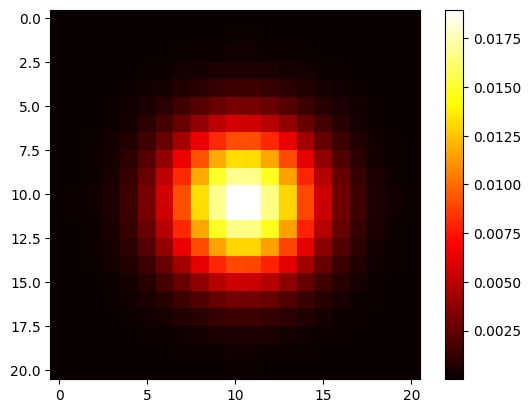
\includegraphics[width=0.7\textwidth]{imgs/norm_esp.png}
    \caption{Visualização do filtro Gaussiano no domínio do espaço}
    \label{fig:norm_esp} 
\end{figure}

Derivando a equação \ref{norm_eq} em relação a $x$ e a $y$, obtemos então as seguintes equações, também definidas sobre o mesmo grid criado anteriormente:

\begin{equation}
    \frac{\partial G}{\partial x}(x,y) = -\frac{x}{\sigma^3 \sqrt{2\pi}} \exp\left(-\frac{x^2 + y^2}{2\sigma^2}\right)
    \label{norm_eq_x}
\end{equation}

\begin{equation}
    \frac{\partial G}{\partial y}(x,y) = -\frac{y}{\sigma^3 \sqrt{2\pi}} \exp\left(-\frac{x^2 + y^2}{2\sigma^2}\right)
    \label{norm_eq_y}
\end{equation}

Então, os filtros foram normalizados com a normalização L2, que é uma técnica essencial para garantir que o filtro preserve a energia (ou magnitude geral) da imagem ao longo da transformação. Especificamente, a normalização pela norma L2 é definida como:

\[
\text{filter} \leftarrow \frac{\text{filter}}{\sqrt{\sum (\text{filter})^2}}
\]

Usando o método \textit{fft} da biblioteca \texttt{Numpy}, os filtros discretos, determinados pelas equações \ref{norm_eq}, \ref{norm_eq_x} e \ref{norm_eq_y}, foram transformados para o domínio da frequência através da Transformada de Fourier. Com isso, foi possível plotar, utilizando a biblioteca \texttt{Matplotlib}, uma visualização de cada um dos filtros no domínio da frequência, conforme apresentado na Figura \ref{fig:fil_freq}.

\begin{figure}[H]
    \centering 
    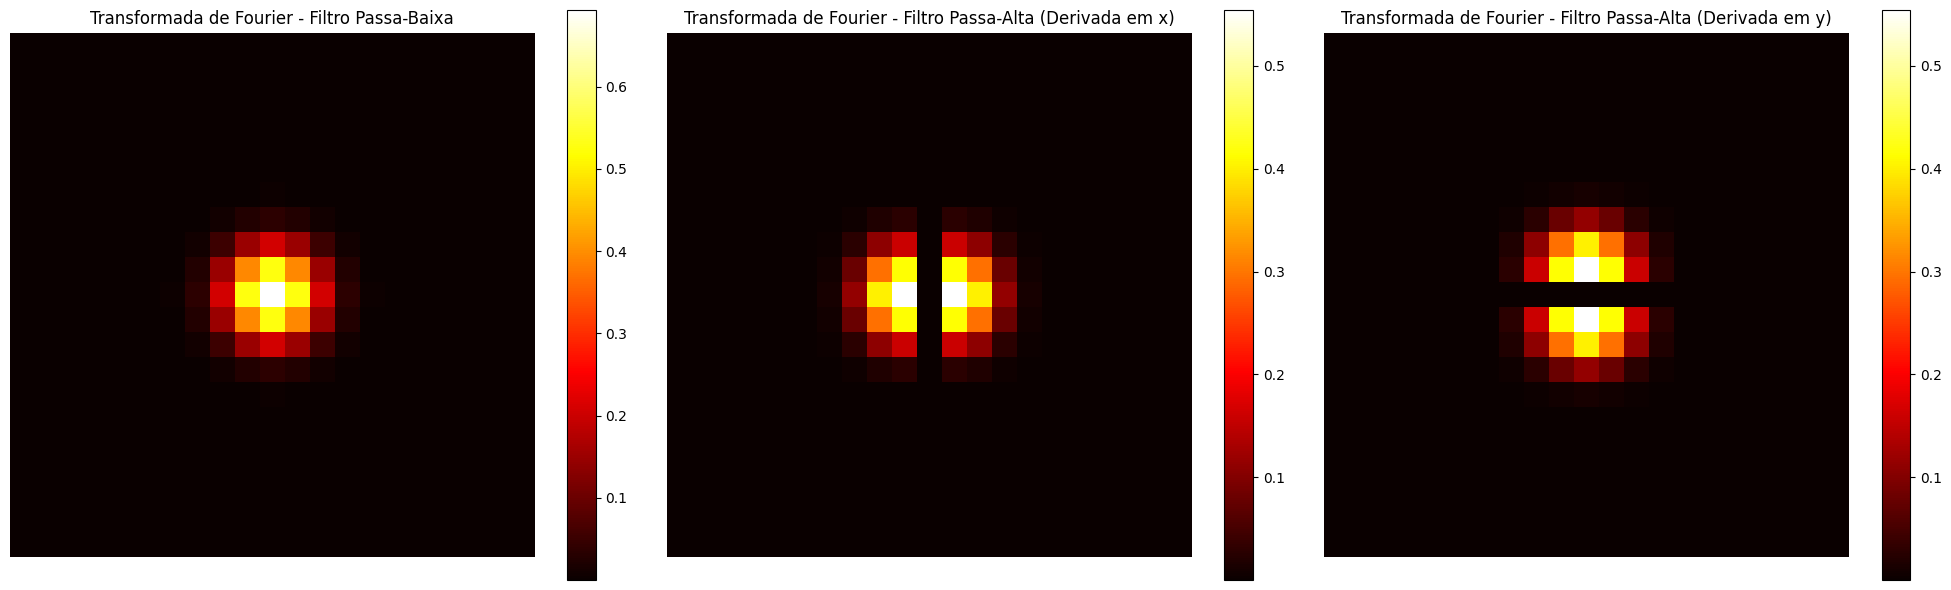
\includegraphics[width=0.95\textwidth]{imgs/filt_four.png}
    \caption{Visualização de cada filtro no domínio da frequência}
    \label{fig:fil_freq} 
\end{figure}

Sabendo que, segundo o teorema da convolução, a multiplicação direta do filtro com a transformada da imagem é equivalente à realização da convolução no domínio do espaço, podemos concluir que a primeira imagem se trata de um filtro passa-baixa, pois as maiores intensidades estão no centro da imagem, correspondendo aos menores valores de frequência. Por outro lado, as outras duas imagens mostram que os filtros são do tipo \textit{high-pass}, já que as frequências próximas de zero nos eixos $x$ e $y$ são anuladas pelos filtros gaussianos parcialmente derivados em relação a $x$ e $y$, respectivamente.

Utilizando a biblioteca \texttt{Skimage} com as classes \textit{io} e \textit{color}, foi carregada uma imagem e convertida para tons de usando a biblioteca \texttt{OpenCV}, com o método \textit{cvtColor}. Em seguida, com o método \textit{convolve} da biblioteca \texttt{Scipy}, aplicamos os filtros a esta imagem. Por padrão, a biblioteca detecta automaticamente a complexidade do cálculo para decidir entre aplicar a convolução diretamente no domínio do espaço ou utilizar o teorema da convolução para operar no domínio da frequência e, posteriormente, retornar ao domínio do espaço. Após esses passos, foi obtido o resultado apresentado na Figura \ref{fig:ney}, que mostra a imagem original seguida das aplicações de cada filtro.

\begin{figure}[H]
    \centering 
    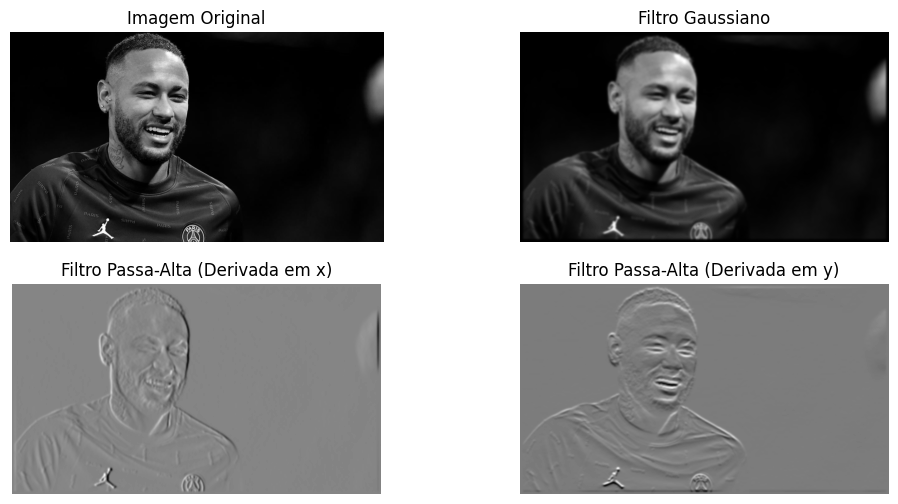
\includegraphics[width=0.95\textwidth]{imgs/ney.png}
    \caption{Visualização da aplicação dos filtros em uma imagem}
    \label{fig:ney} 
\end{figure}

Como podemos observar, os resultados obtidos são consistentes com as características de cada classe de filtro. O filtro passa-baixa realizou uma suavização na imagem, enquanto os filtros do tipo high-pass destacaram as frequências mais atenuantes, geralmente presentes nas bordas dos elementos da imagem. É interessante notar que, no filtro derivado em relação a $x$, houve uma detecção das bordas predominantemente no sentido do eixo $x$, enquanto no filtro derivado em relação a $y$, as bordas foram detectadas no sentido do eixo $y$.


% ===========================================================================================
% ===========================================================================================
% ===========================================================================================
% ===========================================================================================
% ===========================================================================================
% ===========================================================================================
% ===========================================================================================
% ===========================================================================================
% ===========================================================================================

\section{\textbf{Questão 2}}
\noindent \textit{Estude a teoria do PCA para problemas de poucas amostras, onde o número de dados é menor do que a dimensão do espaço de dados. Escolha um banco de dados de imagens, converta as imagens para escala de cinza e aplique a teoria de "PCA para problemas de poucas amostras" para redução de dimensionalidade.}

\begin{enumerate}
    \item[(a)] \textit{Se $\bar{x}$ é a média amostral (centroide do conjunto de dados) e $p_1$ é o componente principal, visualize o resultado da expressão:}
    \[
    x = \bar{x} + \alpha p_1,
    \]
    \textit{onde $\alpha \in \{-\beta \lambda_1, 0, \beta \lambda_1\}$ com $\lambda_1$ sendo o autovalor associado a $p_1$ e $\beta$ um fator escalar.}
    
    \item[(b)] \textit{Estude o espectro da matriz $X^T X$ para realizar a redução de dimensionalidade. Visualize algumas imagens no espaço de dimensão reduzida.}
    
    \item[(c)] \textit{Construa um gerador de imagens usando os $d$ componentes principais escolhidos no item (b).}
\end{enumerate}

\textbf{Resolução:}

Para realizar a redução de dimensionalidade utilizando Análise de Componentes Principais (PCA) em um conjunto de dados onde o número de amostras é inferior à dimensão do espaço dos dados, foi escolhida a base de imagens \textit{originalimages} da FEI Face Database \cite{FEI}. Esta base é composta por 400 imagens faciais frontais, coloridas, de homens e mulheres, sérios e sorridentes, com resolução de $260 \times 360$ pixels. Todos os gráficos e visualizações de imagens foram realizados com a biblioteca \texttt{Matplotlib}. Para o carregamento das imagens, obtidas em \cite{FEI}, foram utilizadas as bibliotecas \texttt{OS} e \texttt{PIL}, que também realizaram a conversão das imagens para arrays \texttt{numpy}, o formato desejado para os cálculos subsequentes. Antes da conversão para arrays, através da biblioteca \texttt{OpenCV}, com o método \textit{cvtColor}, as imagens foram convertidas para tom de cinza. A figura \ref{fig:FEI} mostra alguns exemplos de imagens presentes neste banco de dados já convertidas para tom de cinza.

\begin{figure}[H]
    \centering 
    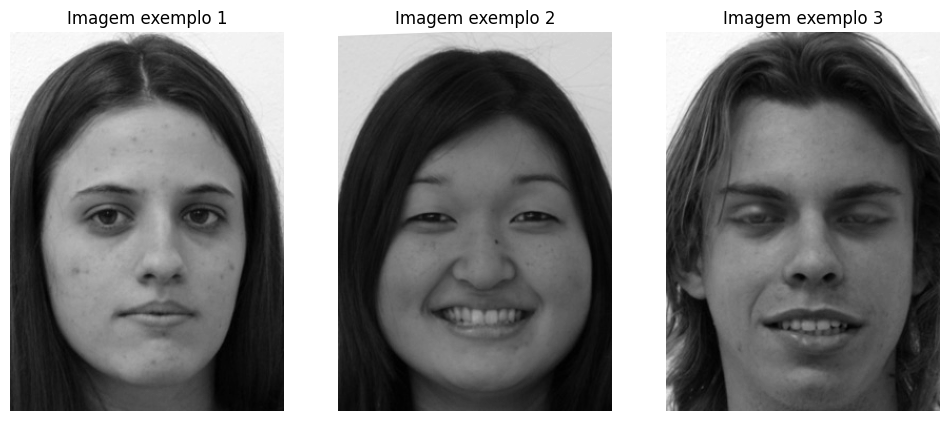
\includegraphics[width=0.8\textwidth]{imgs/FEI.png}
    \caption{Imagens geradas para o item (a)}
    \label{fig:FEI} % cria um rótulo para referência no texto
\end{figure}

Como este é um problema com poucas amostras em relação à dimensionalidade dos dados, para o cálculo da matriz $P_{PCA}$, com o objetivo de minimizar a perda de informação das imagens ao reduzir sua dimensionalidade, seguimos os passos descritos em \cite{miranda2023abordagens}. Aqui, $X$ representa a matriz de dados já vetorizada: 

\begin{enumerate}
    \item Calculo da matriz $\tilde{X}$ de dados centralizados pela expressão \[\tilde{X} = \begin{bmatrix}
    \tilde{x}_1^T \\
    \tilde{x}_2^T \\
    \vdots \\
    \tilde{x}_N^T
    \end{bmatrix}
    \in {R}^{N \times n},\]
    onde N é o número de amostras e n é a dimensão do espaço de dados (neste caso, $360 \cdot 260=93600$) e cada $\tilde{x}_i$ é centralizado da forma $\tilde{x}_i=x-\bar{x}$, onde $\bar{x}$ é a média dos dados.
    \item Resolução do problema de autovalores e autovetores para a matriz $\dfrac{1}{N} \tilde{X} \tilde{X}^T \in {R}^{N \times N}$:
    \[
    \ \dfrac{1}{N}\tilde{X} \tilde{X}^T v_i = \lambda_i v_i,
    \]
    \item Calculo dos vetores $\omega_i = \tilde{X}^T v_i, \quad i = 1, 2, \dots, N.$
    \item Normalização dos vetores $\omega_i$ para obter os autovetores da matriz de covariância $S = \dfrac{1}{N} \tilde{X}^T \tilde{X}$:
    \[
    a_i = \frac{\omega_i}{\|\omega_i\|} = \frac{\tilde{X}^T v_i}{\|\tilde{X}^T v_i\|}.
    \]
\end{enumerate}

Os autovetores obtidos ao final desse processo, ordenados em ordem decrescente em relação aos respectivos autovalores, são as colunas da matriz $P_{PCA}$ que queríamos. 

O cálculo dos autovetores e autovalores da matriz foi realizada através da função \texttt{np.linalg} e a multiplicação de matrizes foi calculada por meio da função \texttt{np.dot}, ambas presentes na biblioteca científica \texttt{Numpy}. Foi criada uma classe para a criação de todos os métodos necessários para a realização desta questão.

Para o item (a), o resultado da expressão $\mathbf{x} = \bar{\mathbf{x}} + \alpha \mathbf{p}_1$, com $\alpha \in \{-\beta\sqrt{\lambda_1}, 0, \beta\sqrt{\lambda_1}\}$, com $\beta=0.8$, resultou nas imagens presentes na figura , onde $\lambda_1 = 51139693.992$ é o autovalor correspondente à componente principal $\mathbf{p_1}$. A legenda coeficiente 1 se trata do valor $-\beta\sqrt{\lambda_1}$, o coeficiente 2 é 0 e o coeficiente 3 é $\beta\sqrt{\lambda_1}$. 

\begin{figure} [H]
    \centering 
    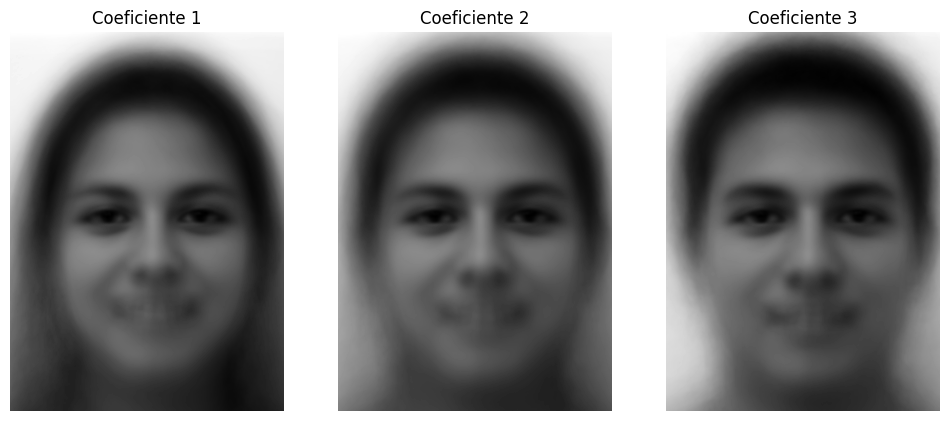
\includegraphics[width=0.8\textwidth]{imgs/2-a.png}
    \caption{Imagens geradas para o item (a)}
    \label{fig:a} % cria um rótulo para referência no texto
\end{figure}

As imagens revelaram que a principal componente capturou predominantemente o fundo das fotos, um elemento comum a todas elas. Isso resultou na aproximação das faces individuais à "face média" derivada do conjunto de imagens.

Para o item (b), foram calculados os autovalores da matriz \( S = \frac{1}{N} \tilde{X}^T \tilde{X} \), que posteriormente foram ordenados em ordem decrescente. Com base nesses valores, foi plotado o gráfico da variância explicada, tanto individual quanto acumulada, com o objetivo de analisar a contribuição de cada autovalor na representação do conjunto de dados e identificar as principais componentes.

A variância acumulada foi obtida pela soma sequencial dos autovalores em ordem decrescente. Quando essa soma atingiu 95\% do total dos autovalores, determinou-se que 95\% da energia total estavam representados por esse subconjunto. Com base no gráfico da Figura \ref{fig:var}, foi decidido reduzir a dimensionalidade para as 110 primeiras componentes, uma vez que essas já representavam mais de 95\% da energia total dos autovalores.

\begin{figure} [h]
    \centering 
    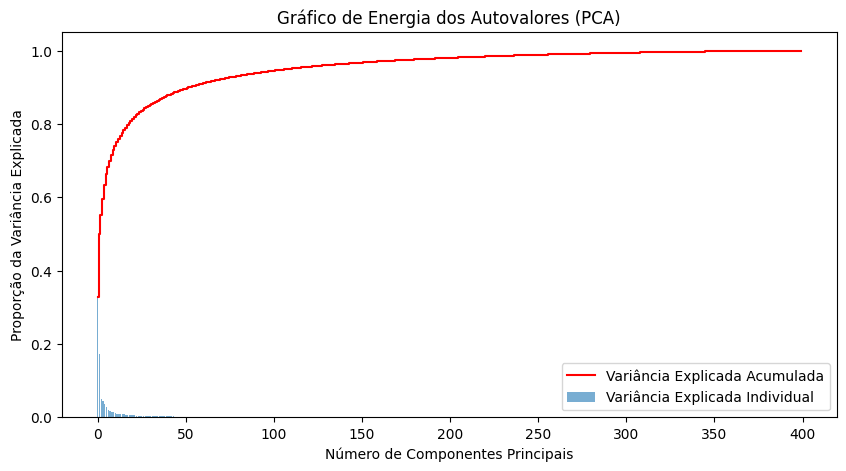
\includegraphics[width=0.8\textwidth]{imgs/var.png}
    \caption{Gráfico de energia dos autovalores}
    \label{fig:var} % cria um rótulo para referência no texto
\end{figure}

Foi então aplicado o truncamento multiplicando a matriz $P_{PCA}$ por $I_{110}$, onde I tem dimensão $400\times 400$, que é o tamanho das colunas da matriz $P_{PCA}$, mas tem até os primeiros 110 números da diagonal preenchido por 1, e todo o resto por 0. Para visualizar então como ficaram as imagens após essa redução, foi realizado o cálculo $X \cdot P_{PCA} \cdot P_{PCA}^T$, obtendo então as imagens presentes na figura \ref{fig:com} com a comparação com suas originais. 

\begin{figure} [H]
    \centering 
    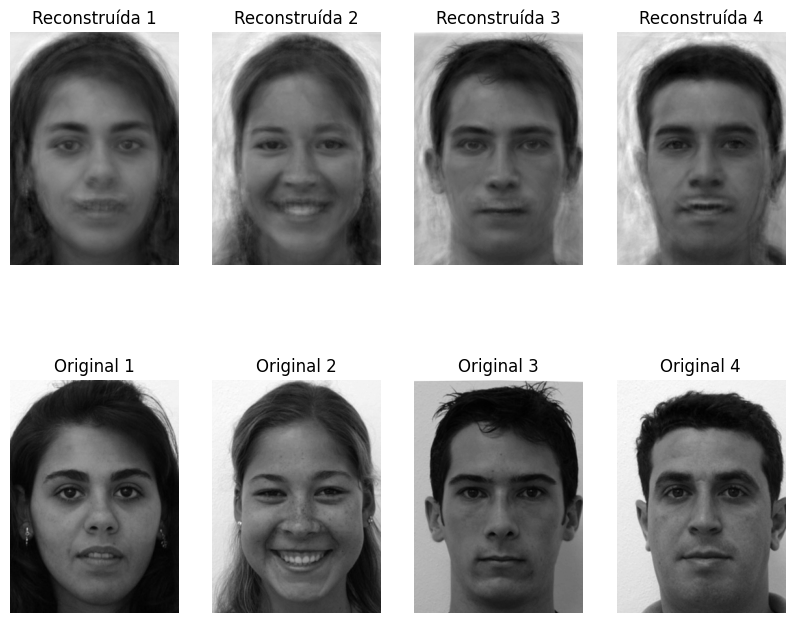
\includegraphics[width=1.0\textwidth]{imgs/comparacao-imagens.png}
    \caption{Comparação reconstruída e original}
    \label{fig:com} % cria um rótulo para referência no texto
\end{figure}

Nas imagens, é notada a redução de qualidade e nitidez em relação à imagem original, mas de forma que as faces ainda mantiveram seus traços e podem ser reconhecidas.

Para o item (c), na construção do gerador de imagens, foi realizada a seguinte operação:

\begin{equation}
\mathbf{x} = \bar{\mathbf{x}} + \sum_{i=1}^{110}  \beta_i \sqrt{\lambda_i} \mathbf{p}_i    
\end{equation}

Onde:

\begin{itemize}
    \item $\lambda_i$ é o i-ésimo autovalor;
    \item $\bar{\mathbf{x}}$ é a média amostral das imagens;
    \item $\mathbf{p}_i$ é o autovetor associado ao i-ésimo autovalor;
    \item $\beta_i$ é o i-ésimo coeficiente, que foi sorteado entre 0 e 1, com o uso de uma distribuição de probabilidade uniforme disponibilizada pela \texttt{Numpy} denominada \texttt{np.random.uniform}.
\end{itemize}

Obtivemos, como resultado, as quatro imagens de novas faces ilustradas na Figura~\ref{fig:ger}. As diferenças entre as imagens geradas devem-se ao fato de que os coeficientes $\beta$ eram sorteados aleatoriamente a cada iteração do cálculo da equação, resultando em variações nas características faciais.

\begin{figure} [H]
    \centering 
    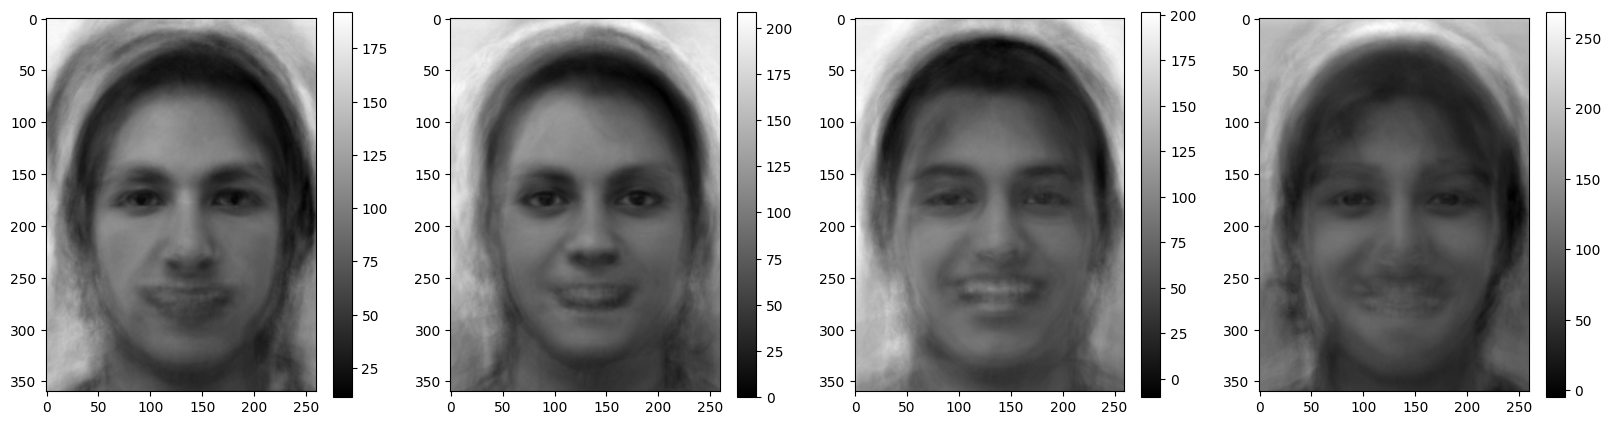
\includegraphics[width=0.95\textwidth]{imgs/gerador.png}
    \caption{Imagem gerada pelas 110 primeiras componentes}
    \label{fig:ger} % cria um rótulo para referência no texto
\end{figure}

Ao realizar várias gerações, foram observadas faces com características marcantes e variadas, como diferentes formatos de lábios, sobrancelhas e narizes. Em um dos testes, embora a imagem não esteja incluída neste trabalho, foi possível gerar uma pessoa usando óculos, enquanto outras não apresentavam esse acessório. Além disso, em comparação com o item (a), percebe-se que, quanto mais componentes principais são utilizadas, mais informações e detalhes são incorporados às imagens geradas.

% ========================================================================================
% ===========================================================================================
% ===========================================================================================
% ===========================================================================================
% ===========================================================================================
% ===========================================================================================
% ===========================================================================================
% ===========================================================================================
% ===========================================================================================
% ===========================================================================================

\section{\textbf{Questão 3}}
\noindent \textit{Escolha uma base de imagens \( D \), converta as imagens para tons de cinza. Separe \( D \) em dois subconjuntos disjuntos \( D_{tr} \) e \( D_{te} \).}

\begin{enumerate}
    \item[(a)] \textit{Calcule o \emph{“PCA para problemas de tamanho de amostra pequeno”} em \( D_{tr} \).}
    \item[(b)] \textit{Estude o espectro da matriz \( R = \frac{1}{N} X^T X \) para realizar a redução de dimensionalidade.}
    \item[(c)] \textit{Aplique o PCA em \( D_{te} \) e compare a eficiência de compressão com o DCT.}
\end{enumerate}

\textbf{Resolução:}

Para a realização desta questão, foi utilizada a mesma base de imagens \textit{originalimages} da FEI Face Database \cite{FEI}. As imagens foram novamente convertidas para tons de cinza e vetorizadas para aplicação do PCA.

Com o objetivo de dividir os dados em conjuntos de treino e teste, utilizou-se o método \texttt{train\_test\_split} da biblioteca \texttt{Sklearn}, com o parâmetro \texttt{test\_size} configurado para 20\%, garantindo que 80\% das amostras fossem destinadas ao treinamento.

Utilizando a classe e as funções criadas no exercício anterior, o PCA foi treinado com o conjunto de treinamento, e o espectro da matriz \( R = \frac{1}{N}X^TX \) foi analisado para realizar a redução de dimensionalidade. Foram calculados os autovalores da matriz \(R\), que foram ordenados em ordem decrescente. Com base nesses valores, foi plotado o gráfico da variância explicada acumulada, visando analisar a contribuição de cada autovalor na representação do conjunto de dados e identificar as principais componentes. 

Os resultados mostraram que as 99 primeiras componentes já representavam 95\% da variância dos dados, conforme ilustrado na Figura~\ref{fig:var2}. Assim, foi realizado o truncamento, multiplicando a matriz \( P_{\text{PCA}} \) por \( I_{99} \), utilizando as funções desenvolvidas na questão anterior.

\begin{figure} [h]
    \centering 
    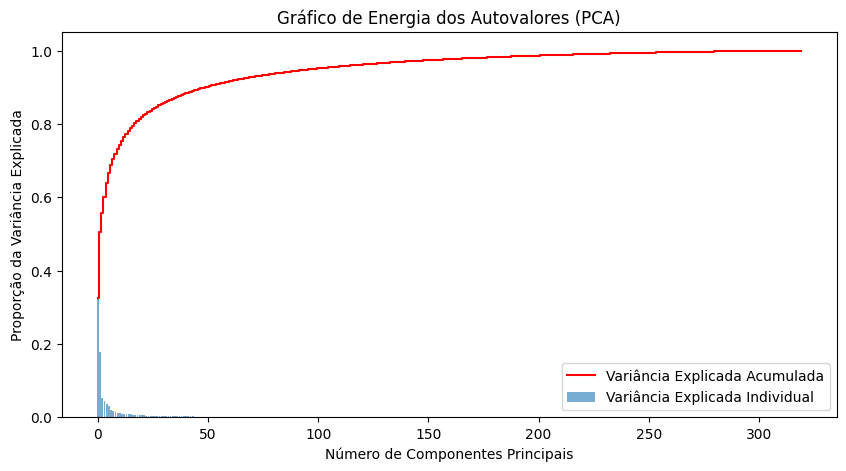
\includegraphics[width=0.8\textwidth]{imgs/var2.png}
    \caption{Gráfico de energia dos autovalores}
    \label{fig:var2} % cria um rótulo para referência no texto
\end{figure}

Logo, foi aplicado o PCA no conjunto de testes e realizada sua reconstrução, utilizando a matriz \( P_{\text{PCA}} \) truncada e sua transposta.

Com a biblioteca \texttt{Scipy}, utilizando a classe \textit{fftpack}, foi calculada a DCT (Transformada Discreta de Cosseno) deste conjunto de testes, usando a equação de acordo com a aula4.pdf:

\begin{equation}
c(k, n) = 
\begin{cases} 
\frac{1}{\sqrt{N}}, & \text{se } k = 0, \quad 0 \leq n \leq N - 1, \\[10pt]
\sqrt{\frac{2}{N}} \cos\left(\frac{\pi (2n + 1) k}{2N}\right), & \text{se } 1 \leq k \leq N - 1, \quad 0 \leq n \leq N - 1.
\end{cases}
\end{equation}

Essa equação é especificada como parâmetro $\text{type}=2$ na função \textit{dct} usada para a aplicação e \textit{idct} para a reconstrução, na classe \textit{fftpack}. 

Para o truncamento, foram calculados os valores absolutos das intensidades dos pixels de cada imagem, ordenados em ordem decrescente, e realizada a soma cumulativa desses valores. Quando a soma acumulada atingiu uma determinada porcentagem da soma total, todas as coordenadas da DCT com valores abaixo desse limite foram zeradas, já que as componentes mais importantes na DCT correspondem às maiores intensidades.

Considerando que o PCA reduziu as imagens, que originalmente tinham dimensão \( 260 \times 360 = 93.600 \), para 400 componentes e, após o truncamento, para 99 componentes, foram realizadas duas abordagens para a seleção dessa porcentagem na DCT:

\begin{enumerate}
    \item Taxa igual a \( \dfrac{99}{400} \), correspondente à proporção de componentes retidas após o truncamento do PCA sobre as 400 componentes principais iniciais;
    \item Taxa igual a \( \dfrac{99}{93.600} \), que representa a redução total de componentes em relação à dimensão original das imagens.
\end{enumerate}

O resultado da reconstrução das imagens pelo PCA e pela DCT está presente nas figuras \ref{fig:pca_dct1} e \ref{fig:pca_dct2}, onde a primeira figura se trata da redução da DCT com a porcentagem \( \dfrac{99}{400} \) e a segunda com a porcentagem \( \dfrac{99}{93.600} \).

\begin{figure} [H]
    \centering 
    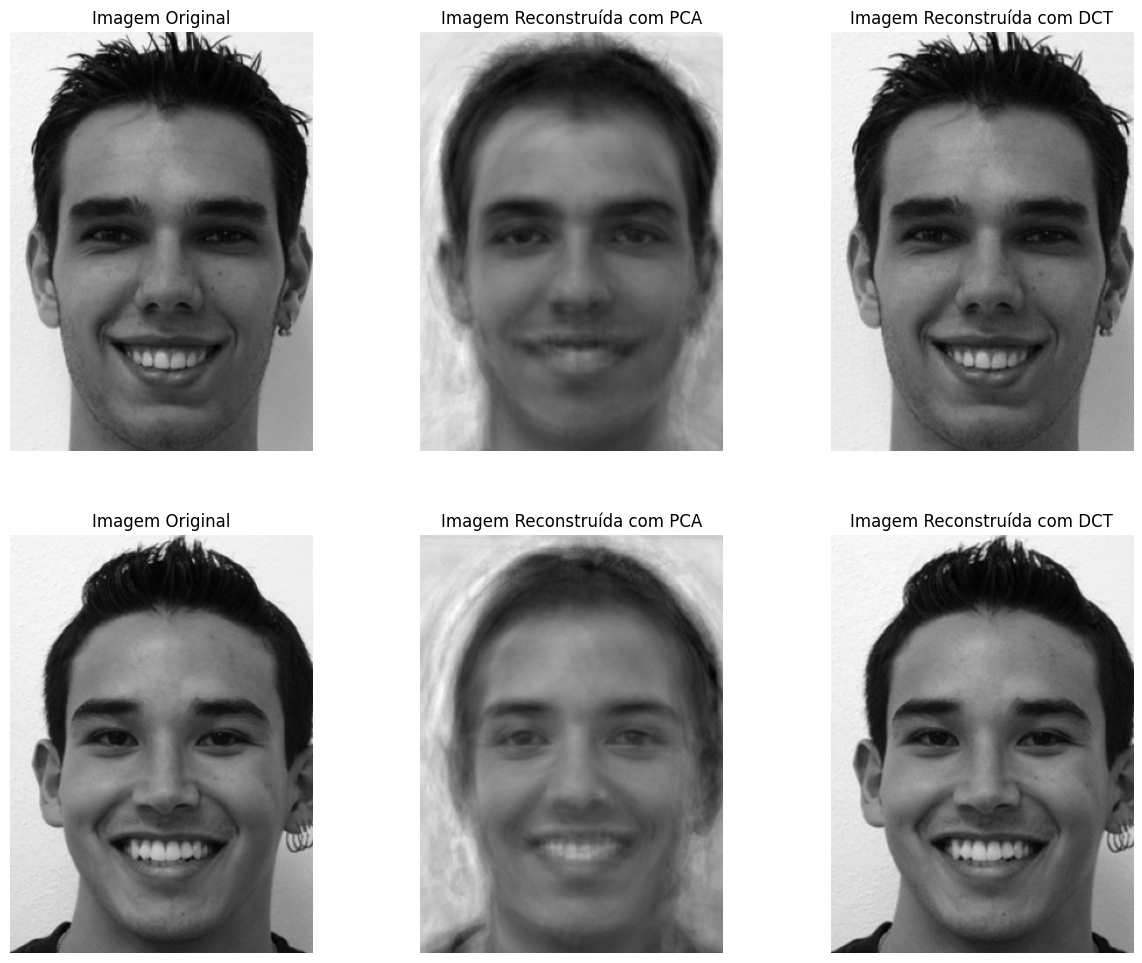
\includegraphics[width=0.7\textwidth]{imgs/pca_dct_1.png}
    \caption{Imagens Reconstruídas - Primeira proporção}
    \label{fig:pca_dct1} % cria um rótulo para referência no texto
\end{figure}

\begin{figure} [H]
    \centering 
    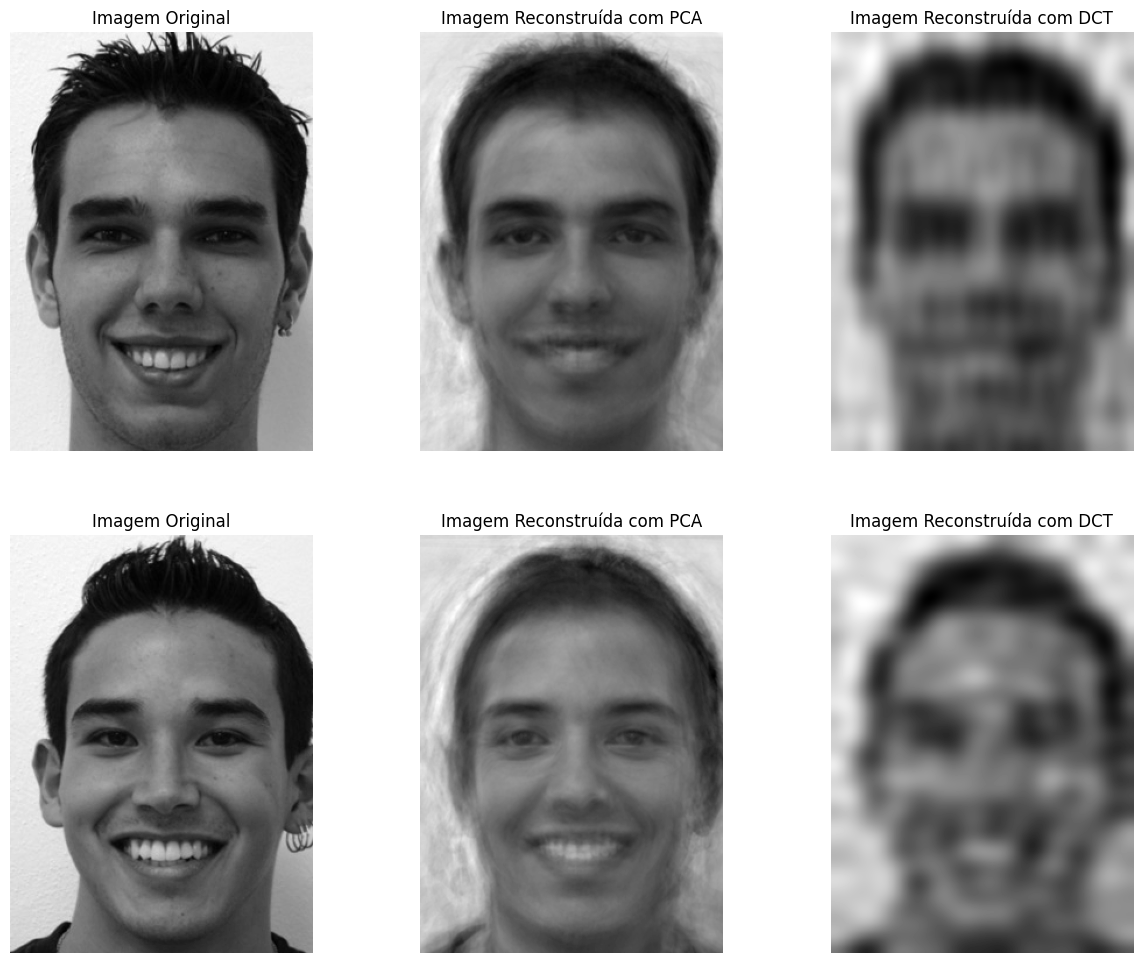
\includegraphics[width=0.7\textwidth]{imgs/pca_dct2.png}
    \caption{Imagens Reconstruídas - Segunda proporção}
    \label{fig:pca_dct2} % cria um rótulo para referência no texto
\end{figure}

As reconstruções evidenciam que, para efeito de comparação de eficiência entre a reconstrução pelo PCA e pela DCT, considerando a primeira proporção, a DCT apresenta uma grande vantagem, gerando uma imagem muito mais próxima da original em comparação com o PCA. Já para a segunda proporção, embora seja possível identificar na reconstrução da DCT que se tratam de rostos, a reconstrução do PCA apresentou um desempenho superior. Logo, podemos concluir que, com apenas 99 componentes, o PCA conseguiu preservar melhor a informação original, superando a DCT em termos de eficiência na conservação de informações com menos componentes.

% ========================================================================================
% ===========================================================================================
% ===========================================================================================
% ===========================================================================================
% ===========================================================================================
% ===========================================================================================
% ===========================================================================================
% ===========================================================================================
% ===========================================================================================
% ===========================================================================================

\section{Questão 4}

\textit{Escolha oito imagens de uma base de dados de imagens, por exemplo, \( I_1, I_2, \dots, I_8 \). Converta-as para escala de cinza (se necessário) e redimensione para \( N \times N \). Calcule a transformada discreta do seno para cada imagem, denotada por \( V_i \), onde \( i = 1, 2, \dots, 8 \), e os valores absolutos correspondentes \( \text{ABS}(V_i) \), para \( i = 1, 2, \dots, 8 \).}

\begin{itemize}
    \item[(a)] \textit{Concatenate as imagens em uma lista \( I = [I_1, I_2, \dots, I_8] \) e forme a lista \\ \( L_{\text{abs}} = [\text{ABS}(V_1), \text{ABS}(V_2), \dots, \text{ABS}(V_8)] \). Calcule as características estatísticas para \( L_{\text{abs}} \). Exemplos: valor mínimo, valor máximo, média, desvio padrão, histograma, etc. Discuta os resultados.}
    \item[(b)] \textit{Aplique o resultado do item 4(a) para projetar uma estratégia de redução de dimensionalidade. Visualize alguns resultados da reconstrução.}
\end{itemize}

\textbf{Resolução:}

Para a realização deste exercício, foram escolhidas 8 imagens da mesma base de imagens \textit{originalimages} da FEI Face Database \cite{FEI}. As imagens foram novamente convertidas para tons de cinza e vetorizadas. Além disso, elas foram transformadas em quadradas, simplesmente cortando as imagens com o uso do array \texttt{Numpy}, de modo que as dimensões se tornaram \( 260 \times 260 \).

Logo após, foi aplicada a transformação seno através do método \textit{dst} da biblioteca \texttt{Scipy}, com o parâmetro \texttt{type=1}, o que significa que a transformação aplicada será condizente com a apresentada na aula4.pdf, dada por:

\begin{equation}
\psi(k, n) = \sqrt{\frac{2}{N + 1}} \sin\left( \frac{\pi (k + 1)(n + 1)}{N + 1} \right), \quad 0 \leq k, n \leq N - 1,
\end{equation}

onde \( N = 260 \) neste caso, gerando o conjunto das imagens transformadas, denotadas por \( V \).

Após isso, utilizando o método \textit{abs} da biblioteca \texttt{Numpy}, foram calculados os valores absolutos de todas as imagens, denotados por \( \text{ABS}(V) \).

Em seguida, com os métodos \textit{mean}, \textit{median}, \textit{std}, \textit{min} e \textit{max} da biblioteca \texttt{Numpy}, foram calculadas as médias, medianas, desvios padrão, valores mínimo e máximo das intensidades dos pixels de cada imagem do conjunto \( \text{ABS}(V_i) \), gerando os dados presentes na Tabela \ref{tab:4}.

\begin{table}[htbp]
\centering
\begin{tabular}{@{}lccccc@{}}
\toprule
\textbf{Imagem} & \textbf{Média} & \textbf{Mediana} & \textbf{Desvio Padrão} & \textbf{Min} & \textbf{Max} \\ \midrule
Imagem 1 & 8.7748 & 1.0253 & 87.3371 & $1.4401 \times 10^{-5}$ & 14926.2605 \\
Imagem 2 & 8.9512 & 1.5361 & 97.2831 & $3.2046 \times 10^{-5}$ & 17381.0742 \\
Imagem 3 & 8.2167 & 1.3179 & 83.0330 & $2.7641 \times 10^{-5}$ & 17053.3512 \\
Imagem 4 & 8.5232 & 1.3155 & 97.3798 & $2.5473 \times 10^{-5}$ & 15056.8867 \\
Imagem 5 & 7.5279 & 0.9699 & 79.0755 & $1.7497 \times 10^{-5}$ & 14301.8414 \\
Imagem 6 & 8.5386 & 1.0917 & 90.3626 & $2.0046 \times 10^{-5}$ & 15674.7976 \\
Imagem 7 & 6.5690 & 0.7710 & 83.5264 & $9.1508 \times 10^{-6}$ & 11966.9477 \\
Imagem 8 & 8.6343 & 1.5474 & 95.8161 & $1.7381 \times 10^{-5}$ & 14666.8876 \\ \bottomrule
\end{tabular}
\caption{Estatísticas das imagens.}
\label{tab:4}
\end{table}

Além disso, a fim de visualizar melhor a distribuição das intensidades no domínio da frequência, foi plotado o histograma do valor absoluto do logaritmo dessas intensidades. Para isso, foi utilizada a biblioteca \texttt{Matplotlib} com o método \textit{hist}, configurado com o parâmetro \textit{density} igual a true, para que fosse exibida a frequência relativa das intensidades. Os resultados estão ilustrados na figura \ref{fig:4_hist}, que mostra o gráfico para cada uma das imagens. Em imagens transformadas para o domínio da frequência (como usando a DST), há picos muito altos em baixas frequências e valores muito baixos em altas frequências. O uso do logarítmico reduz a diferença entre esses extremos, tornando os detalhes nas regiões de menor amplitude mais visíveis. Logo, valores pequenos são destacados sem serem "esmagados" pelos valores mais altos. Isso é útil, por exemplo, para identificar ruídos ou padrões em altas frequências que poderiam ser negligenciados em uma escala linear. Por isso a adoção da escala logarítima para plotar os histogramas.

\begin{figure}[H]
    \centering
    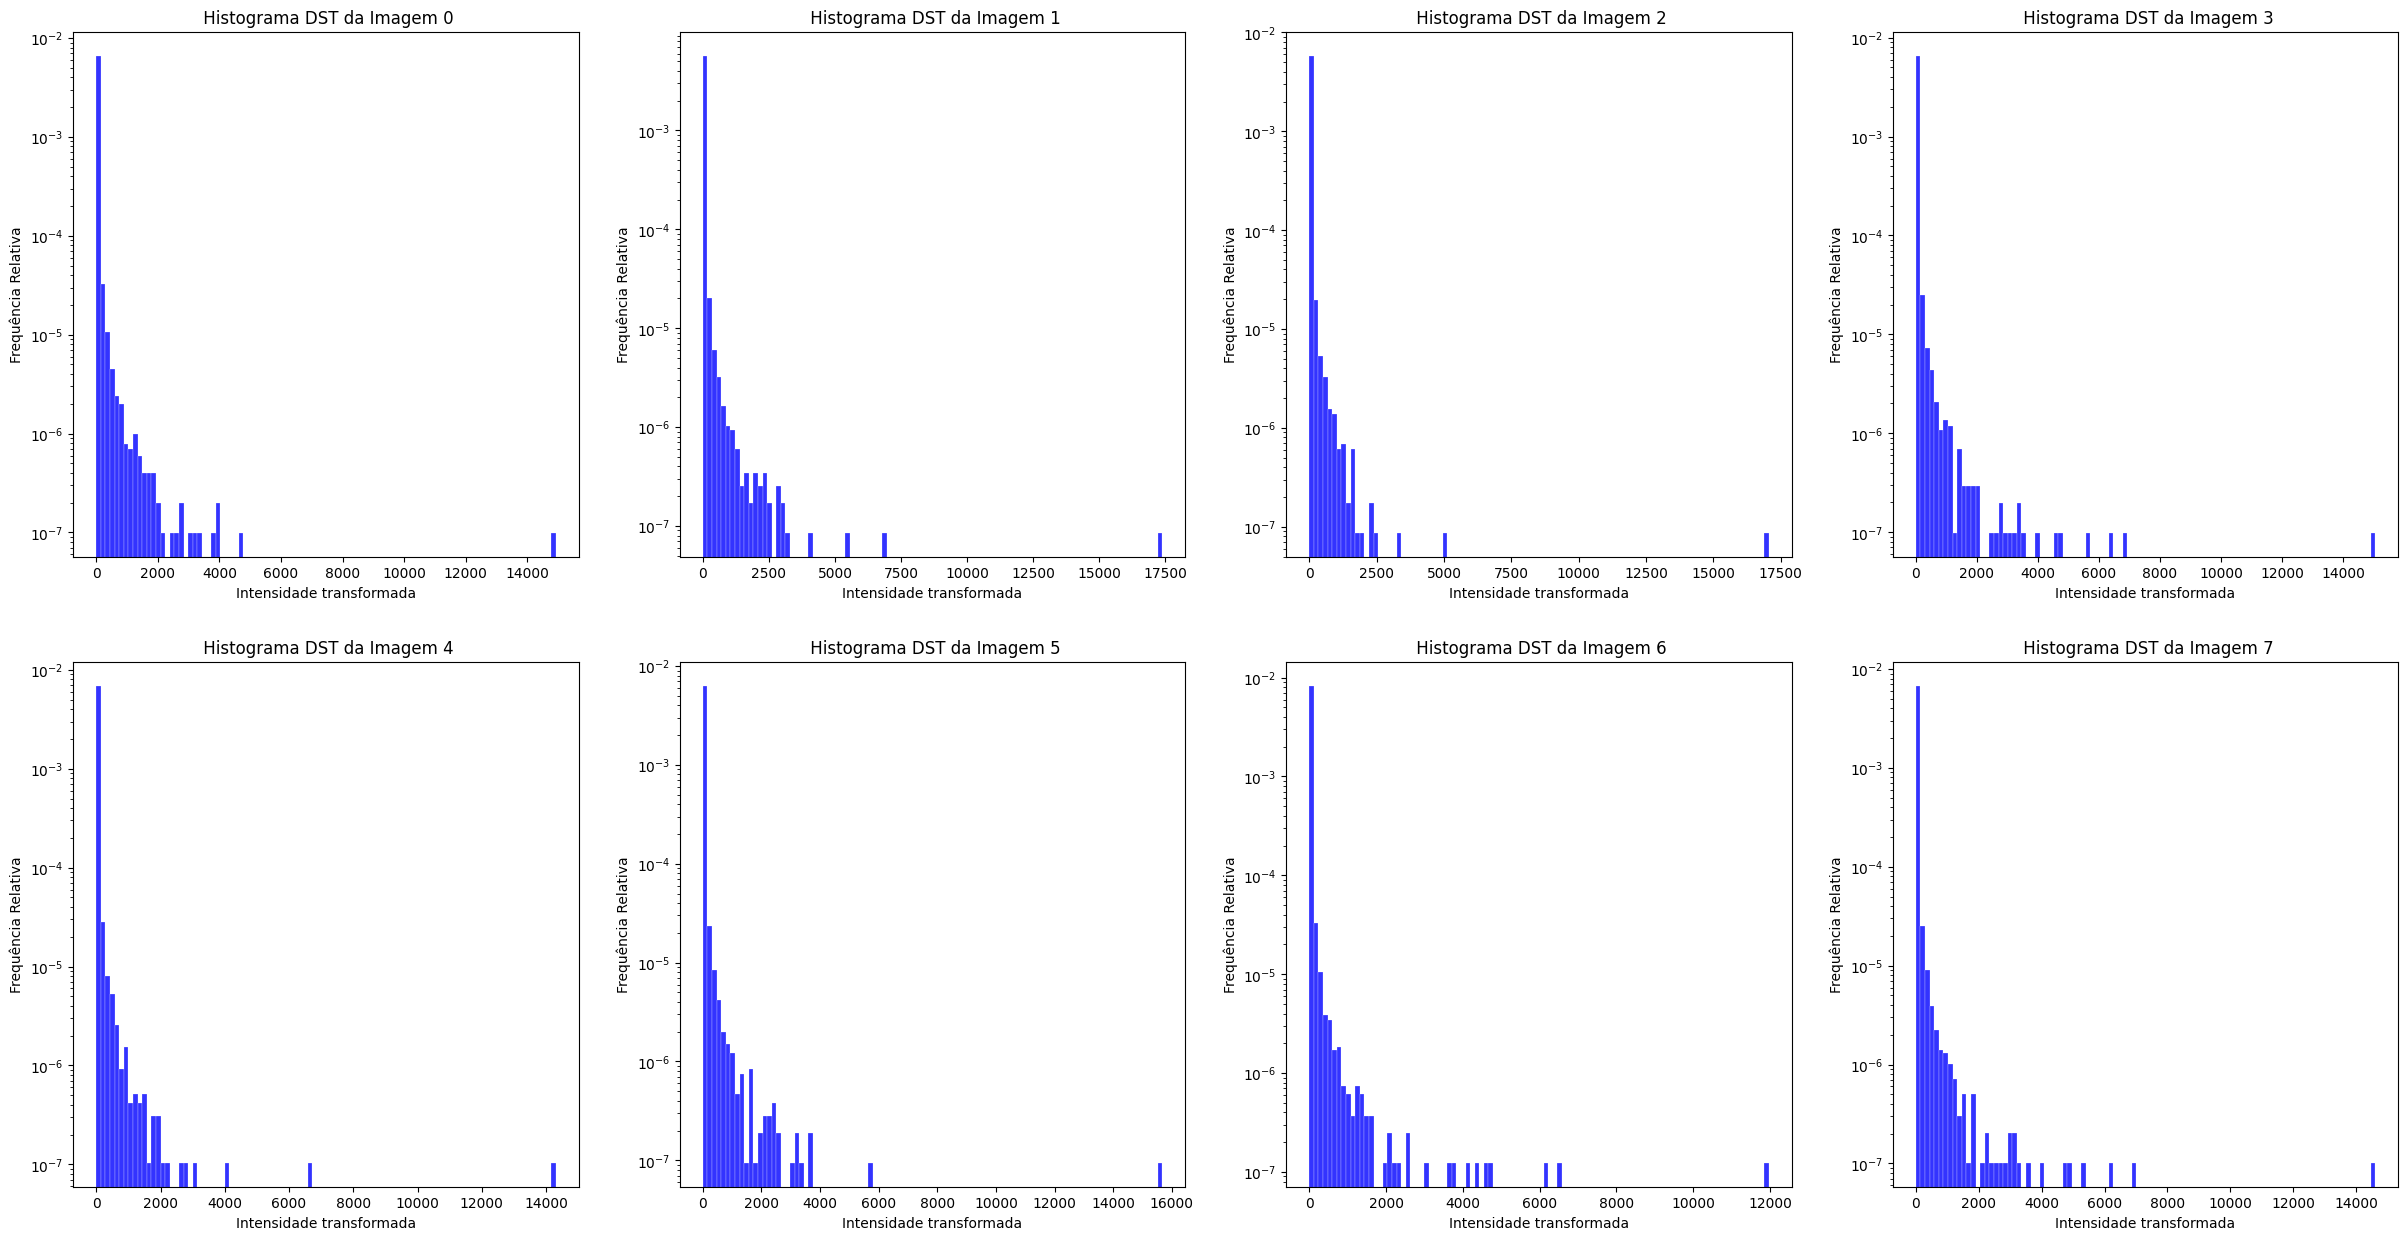
\includegraphics[width=0.95\textwidth]{imgs/4_hist.png}
    \caption{Histograma do logaritmo das intensidades após a transformação seno (DST).}
    \label{fig:4_hist} % cria um rótulo para referência no texto
\end{figure}

De acordo com as estatísticas obtidas e considerando que, na transformada seno, as intensidades mais altas são as mais importantes, foi desenvolvido o seguinte critério para a redução de dimensionalidade: zerar todas as componentes com valor absoluto fora do intervalo entre a média e o valor máximo, ou seja, abaixo da média. Essa técnica foi adotada também levando em consideração a "grande concentração" de valores próximos à intensidade 0, visto que a média está próximo do valor mínimo e bem distante do valor máximo. Isso pode resultar em uma redução significativa do número de componentes, priorizando as maiores intensidades. Ao realizar essa abordagem, se resultou em média na redução de $87.52\%$ das componentes.

Como forma de comparação, foi utilizado outro método para redução de dimensionalidade na DST. Esse método seleciona a mesma porcentagem de intensidades restantes, mas preservando preferencialmente as intensidades presentes no quadrante superior esquerdo da matriz, onde normalmente estão localizadas a maioria das intensidades mais altas.

Todas as operações necessárias para a realização dessas estratégias foram realizadas com a manipulação dos arrays \texttt{Numpy}.

Os resultados obtidos com as técnicas descritas acima estão apresentados na figura \ref{fig:4_recons}, onde "Reconstruída Q1" refere-se ao método que mantém o quadrante superior esquerdo das intensidades para comparação, e "Min-média" é o método desenvolvido com base na análise estatística.

\begin{figure} [H]
    \centering 
    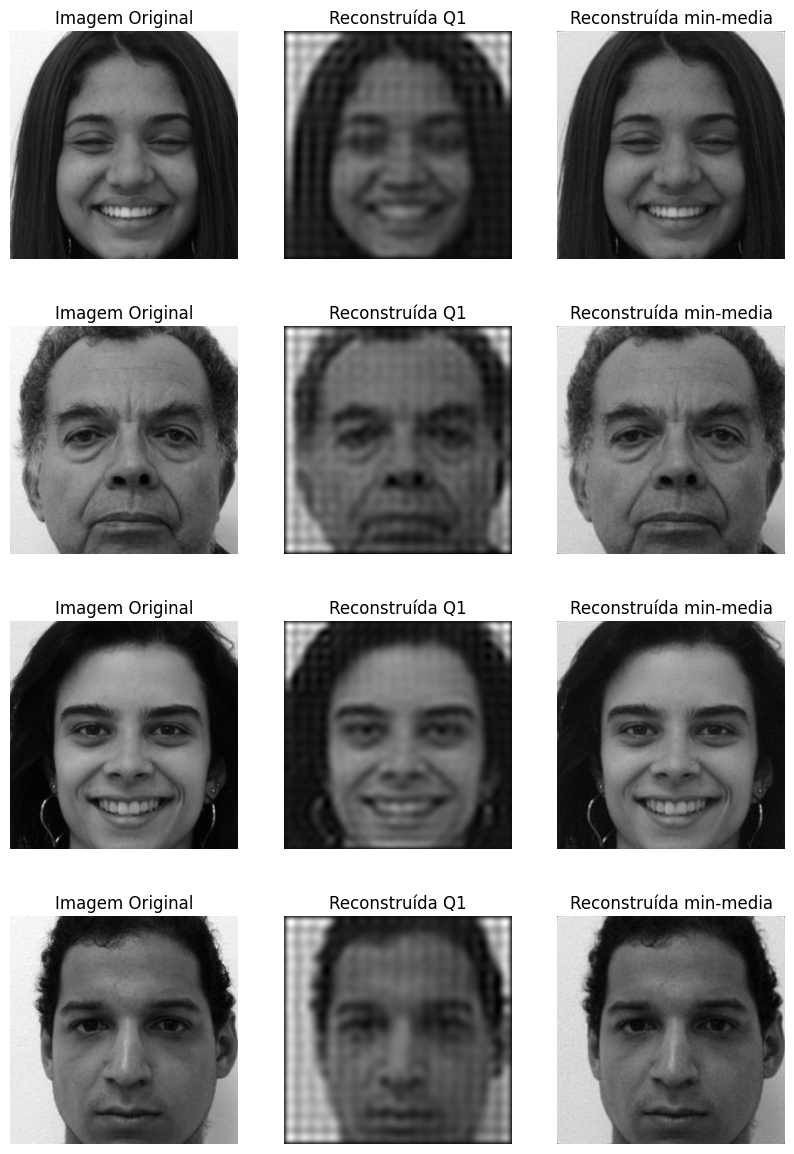
\includegraphics[width=0.7\textwidth]{imgs/4_recons.png}
    \caption{Imagens Reconstruídas - DST}
    \label{fig:4_recons} % cria um rótulo para referência no texto
\end{figure}

Logo, a visualização evidencia como o critério desenvolvido preservou fortemente a qualidade das imagens, apresentando poucas diferenças em relação à imagem original, quando comparado ao outro método, no qual é possível perceber uma perda relevante. Além disso, considerando que, em média, apenas $12,48\%$ das intensidades foram utilizadas para a reconstrução com o método "Min-média", isso demonstra a eficiência do método visto à qualidade das imagens reconstruídas.


\section{Questão 5}

\textit{Agora, aplique o filtro passa-baixa do exercício 1 sobre as imagens na lista 
$I = [I_1, I_2, \ldots, I_8]$ do exercício 4 para obter uma nova lista de 
$I^{\star} = [I^{\star}_1, I^{\star}_2, \ldots, I^{\star}_8]$. 
Calcule $L^{\star}_{\text{abs}}$ e suas estatísticas. Compare os resultados 
com as estatísticas de $L_{\text{abs}}$. Repita o mesmo para o filtro 
passa-alta do exercício 1.
}

\textbf{Resolução:}

Utilizando o filtro passa-baixa Gaussiano construído na questão 1 e o método \textit{convolve} da biblioteca \texttt{Scipy}, foi realizada a convolução no banco de imagens \(I\) definido na questão anterior. De forma análoga, aplicou-se o filtro passa-alta, que considera a derivada do filtro Gaussiano em relação à variável \(x\).

De forma análoga ao procedimento realizado na questão anterior, os dois conjuntos de imagens correspondentes ao cálculo de cada filtro foram transformados para o domínio da frequência utilizando a Transformada Discreta do Seno (DST). Em seguida, foram calculados os valores de média, mediana, desvio padrão, mínimo e máximo para cada imagem. O resultado médio de cada conjunto, após a realização desses cálculos, está apresentado na Tabela \ref{tab:5}.

\begin{table}[h!]
    \centering
    \begin{tabular}{@{}lcccccc@{}}
        \toprule
        \textbf{Filtro} & \textbf{Média} & \textbf{Mediana} & \textbf{Desvio Padrão} & \textbf{Mínimo} & \textbf{Máximo} \\ 
        \midrule
        Original        & 8.2169         & 1.1968           & 89.2267                & 4.3522e-05      & 15121.0049       \\ 
        Passa-baixa     & 2.6108         & 5.4089e-06       & 80.3364                & 8.7297e-13      & 16088.6160       \\ 
        Passa-alta      & 16.5160         & 0.9477           & 179.9396                & 1.4909e-06      & 15394.3647        \\ 
        \bottomrule
    \end{tabular}
    \caption{Estatísticas médias dos conjuntos de imagens aplicados a diferentes filtros}
    \label{tab:5}
\end{table}

Além disso, as figuras \ref{fig:5_hist1} e \ref{fig:5_hist2} ilustram como ficaram o histograma de frequências relativas de cada imagem em cada respectivo conjunto.

\begin{figure}[H]
    \centering
    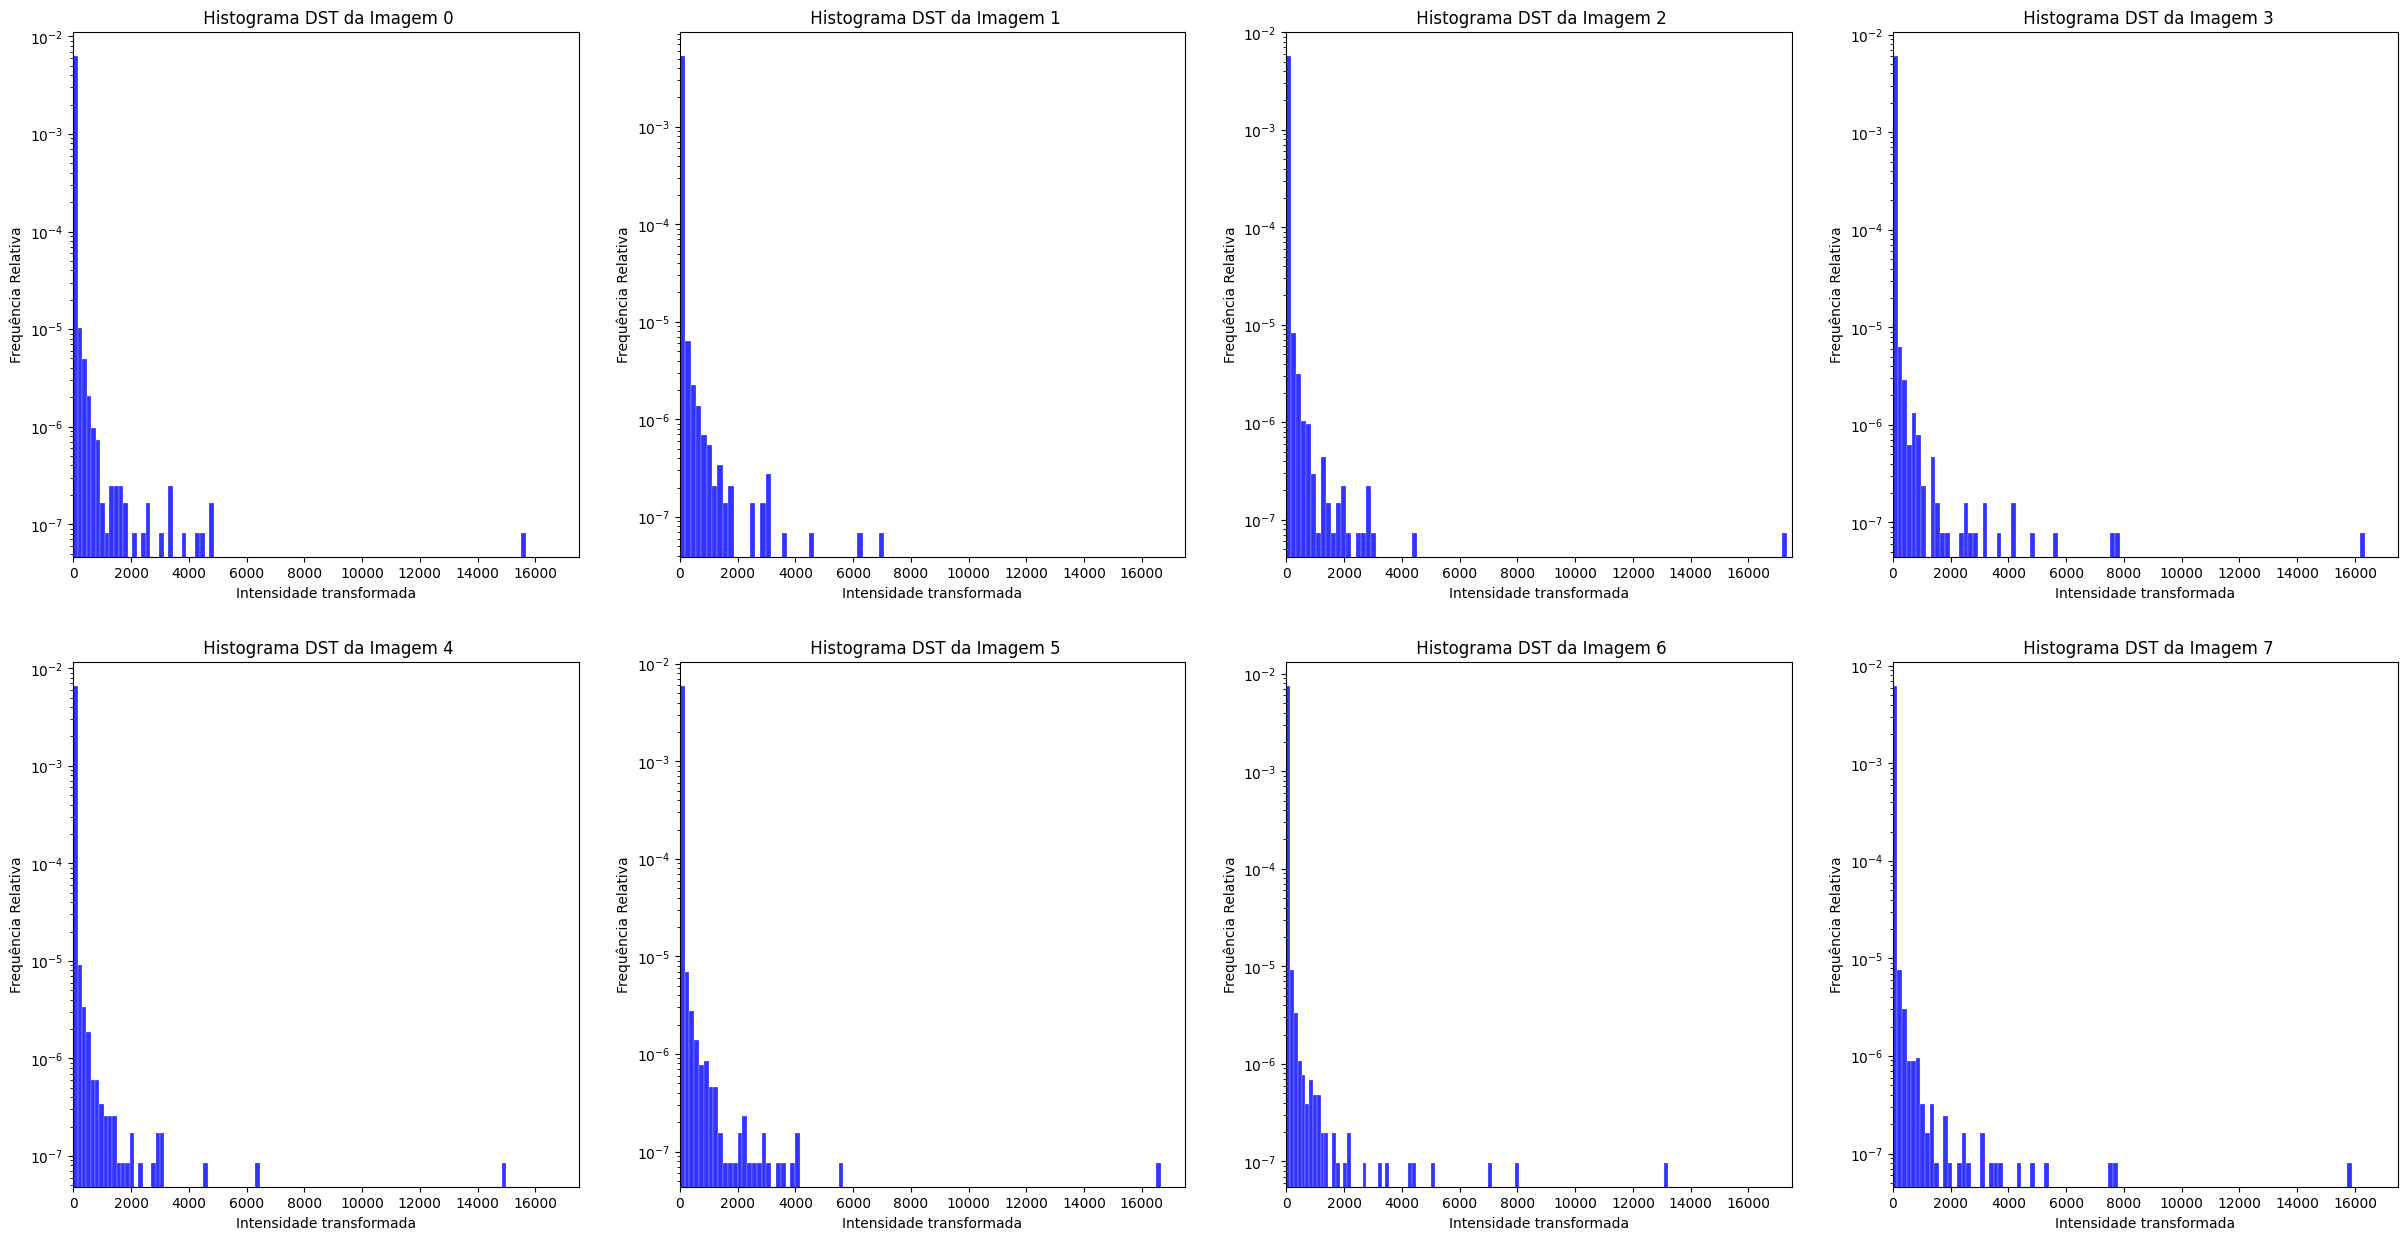
\includegraphics[width=0.95\textwidth]{imgs/5_hist1.png}
    \caption{Histograma do logaritmo das intensidades após a transformação seno (Passa-baixa)}
    \label{fig:5_hist1} % cria um rótulo para referência no texto
\end{figure}

\begin{figure}[H]
    \centering
    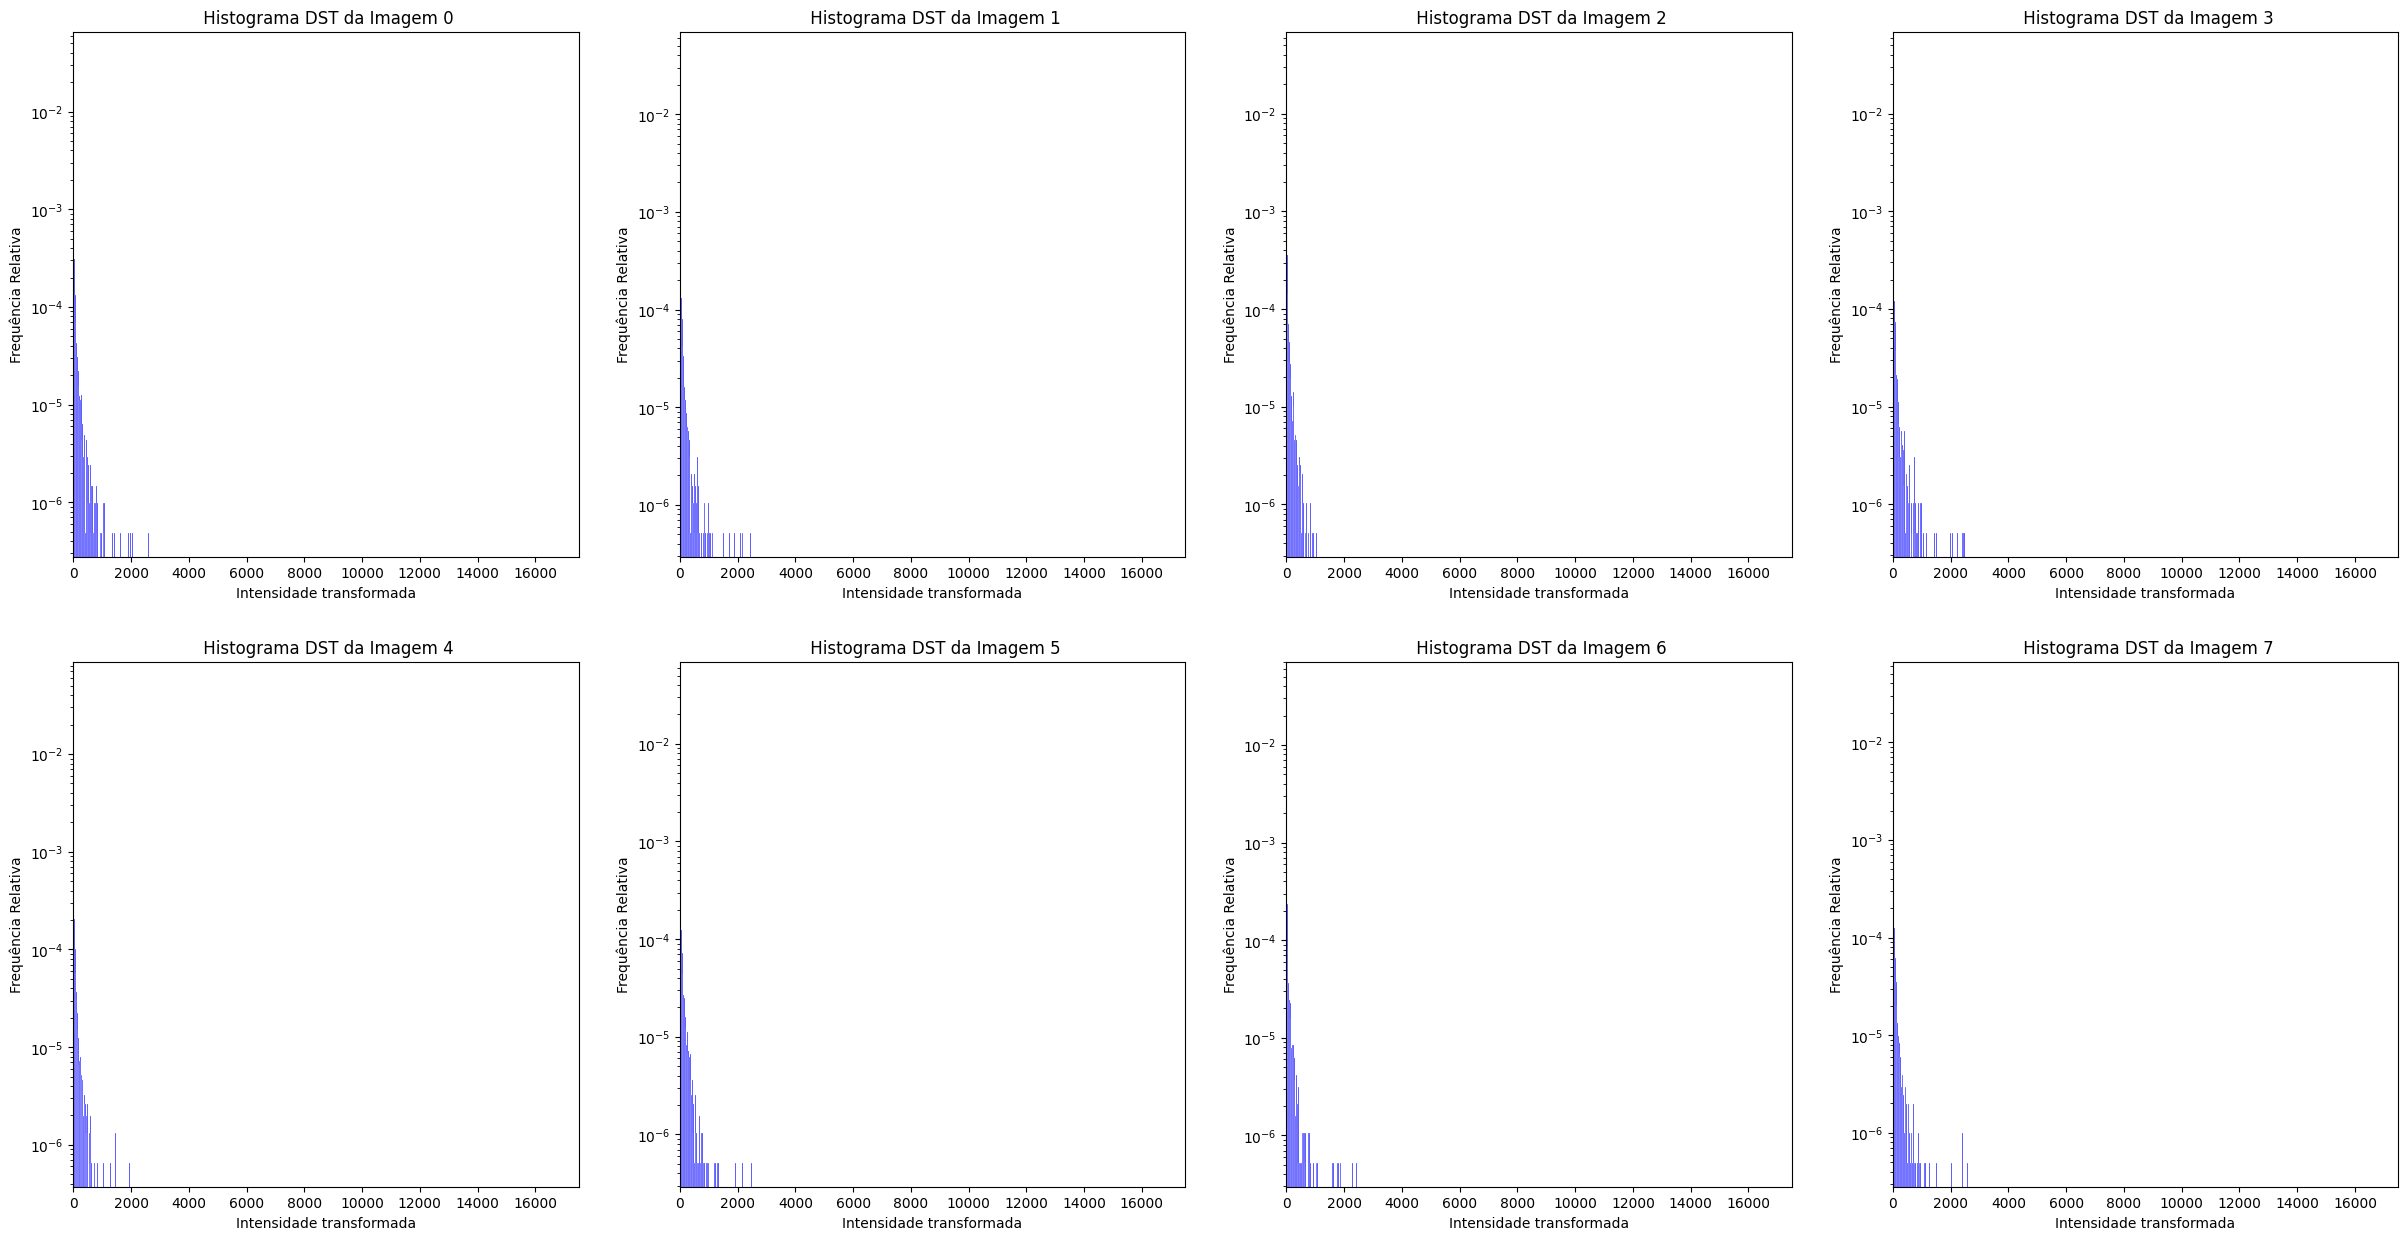
\includegraphics[width=0.95\textwidth]{imgs/5_hist2.png}
    \caption{Histograma do logaritmo das intensidades após a transformação seno (Passa-alta)}
    \label{fig:5_hist2} % cria um rótulo para referência no texto
\end{figure}

Analisando os resultados apresentados na Tabela \ref{tab:5} e nas imagens \ref{fig:5_hist1} e \ref{fig:5_hist2}, podemos observar os efeitos dos filtros passa-baixa e passa-alta aplicados às imagens.

O filtro \textit{passa-baixa}, como esperado, causou uma redução significativa na média das imagens, que passou de 8.2169 no conjunto original para 2.6108. Isso reflete a atenuação das altas frequências, com o filtro suavizando a imagem e removendo detalhes finos de alta frequência. No histograma da imagem filtrada, podemos observar uma concentração de intensidades mais próximas de valores baixos, com uma distribuição de pixels mais comprimida. A mediana foi reduzida para 5.4089e-06, o que sugere que a maioria dos pixels da imagem ficou muito próximo de um valor baixo. O desvio padrão também foi reduzido de 89.2267 para 80.3364, indicando uma diminuição da variação dos valores de intensidade, o que resulta em uma imagem mais homogênea. O valor máximo das intensidades aumentou levemente (de 15121.0049 para 16088.6160), refletindo um leve aumento das componentes de baixa frequência mais intensas, embora ainda dentro de uma faixa limitada.

Em contraste, o filtro \textit{passa-alta} gerou uma mudança mais pronunciada nos dados. A média aumentou substancialmente, de 8.2169 para 16.5160, o que reflete o aumento das componentes de alta frequência e a ampliação dos detalhes da imagem. O histograma da imagem filtrada apresenta uma maior dispersão de intensidades, com picos mais acentuados em torno de valores mais altos, evidenciando o efeito do filtro na amplificação de detalhes agudos. A mediana, que era 1.1968 no original, foi reduzida para 0.9477, mostrando que, apesar do aumento da variabilidade, a distribuição dos pixels foi ligeiramente deslocada para a esquerda. O desvio padrão aumentou consideravelmente, de 89.2267 para 179.9396, como esperado, pois o filtro passa-alta acentua as variações locais na imagem, gerando maior contraste e detalhes. O valor máximo das imagens filtradas, que era 15121.0049, permaneceu relativamente estável (15394.3647), indicando que a intensidade máxima das regiões de alta frequência foi preservada, mas com a redistribuição dos valores dos pixels ao longo de um intervalo mais amplo.

Os histogramas das imagens filtradas são consistentes com os efeitos teóricos dos filtros. No caso do filtro passa-baixa, o histograma mostrou uma forte concentração de pixels em valores baixos, refletindo a suavização da imagem. Já o histograma do filtro passa-alta apresentou uma distribuição mais espalhada, com picos mais pronunciados em áreas de alta intensidade, evidenciando o aumento dos detalhes e a maior variabilidade das intensidades.

Em resumo, os resultados e histogramas confirmam que os efeitos dos filtros no domínio da frequência ocorreram conforme o esperado: o filtro passa-baixa suaviza a imagem, reduzindo a média, a variabilidade e a dispersão dos histogramas, enquanto o filtro passa-alta aumenta os detalhes e o contraste, evidenciado por uma maior dispersão e maior intensidade nos histogramas. A análise dessas métricas confirma que os efeitos dos filtros no domínio da frequência ocorreram conforme o esperado.

\newpage
\bibliography{Bibliografia} 

\end{document}